\section{The Gnomonic and Stereographic Projections}\label{sec:gnom_stereo}
In this section, we'll present some results about two common
projections from the sphere to the plane: the \textit{gnomonic} and
the \textit{stereographic} projections.  We build these results to
show that the convex hull score and the Reock score are not preserved
by any map projection.

\subsection{The Gnomonic Projection}

\zs{old defn 6}

\begin{definition}
	A set $X$ in a metric space is \textbf{convex} if for any pair of
	points $x_1$ and $x_2$ in $X$, the shortest geodesic segment
	connecting $x_1$ and $x_2$ is entirely contained in $X$. 
\end{definition}
In the plane, these geodesic segments are ordinary line segments.  On
the sphere, the geodesics are segments of great circles. In 
particular, this means that on the sphere, caps are 
convex, and in the plane, circular regions are convex.

\zs{old defn 8, lem 3, thm 2,3,4}

\begin{definition}
	The \textbf{gnomonic projection} is the map projection from the
	lower half-sphere to the plane defined by placing the south pole of
	the sphere tangent to the plane at the origin and sending a point
	$p$ on the lower half-sphere to the unique point $q$ in the plane
	which lies on the line in $\mathbb{R}^3$ which passes through the
	center of the sphere, $p$ and $q$.
\end{definition}
Intuitively, the image of a region on the sphere under the gnomonic
projection is the shadow in the plane of that region which is
created when we put the bottom of the sphere at the origin and turn
on a light source at the center of the sphere.

By convention, we will let the sphere be the unit sphere 
centered at $(0,0,1)$.
\zs{do we want to write the explicit parametrization of the gnomonic
projection here? the xy version of it is pretty gross.  the polar
version is less messy.  I don't know if it provides any extra
insight...}
\abn{A figure might be better}

We can observe that the gnomonic projection sends caps centered at the
south pole to circles in the plane centered at the origin, and sends
any segment of a great circle passing through the south pole to a line
segment in the plane passing through the origin.  What may be somewhat
surprising is that it sends \textit{every} convex set on the sphere to
a convex set in the plane.

\begin{lemma} \label{lem:gnomonic_convex}
  Let $\vphi$ be the gnomonic projection, and $U\subset S^2$ a convex 
  set. Then $\vphi(U)$ is convex.
\end{lemma}
\begin{proof}
  To prove this, it suffices to show that the one-dimensional convex
  sets are preserved. In other words, we must show that any segment of 
  a great circle on the sphere is sent to a line segment in the plane.

  Let $p$ be the center of the sphere $S^2$, and let $C\subset S^2$ be
  a geogesic segment in the lower hemisphere.  Note that $C$ is uniquely
  identified by the intersection of $S^2$ with a portion of a plane
  $\mc{P}$ passing through $p$ which is not parallel to the $xy$-plane,  $\mc{P}_{xy}$. Since $\mc{P}$ contains all of the lines passing through $p$ and a point in $C$, by construction, $\vphi(C)\subset \mc{P}\cap
  \mc{P}_{xy}$, and two planes intersect along a line. 

  Since the gnomonic projection is injective, it follows that 
  geodesic segments in $S^2$ cannot be sent to points, and hence 
  must be sent to lines. \zs{do we need this statement?}
\end{proof}




\abn{I'm still hunting down the reference for this theorem. 
Some say it's due to Hartshorne, but I can't find the reference. 
Someone says it's due to von Staudt from the 1850's...}
\begin{theorem} \label{thm:geometric_algebra}
  Let $U$ be some subset of $\mathbb{R}^n$ for $n\geq 2$.  If $f: U\to\R^n$ is 
  bijective and sends line segments  to  line segments, then $f$ is an affine linear 
  transformation.\zs{should try to make work for injective}
\end{theorem}
\begin{proof}
  After possibly translating, we can assume without loss of generality that 
  $0\in U$ and $f(0) = 0$, in which 
  case we must show that $f$ is linear. We write $V = f(U)$. 
  Since $f$ is a bijection  from $U$ to $V$ 
  sending straight lines to straight lines, it follows that 
  if $\mc{P}$ is an affine subspace of $\R^n$, then 
  $f(\mc{P}\cap U)$ must be of the form $\mc{Q}\cap V$, where 
  $\mc{Q}$ is an affine subspace of $\R^n$.
  Additionally, $f$ must preserve intersections of 
  lines, and hence sends coplanar parallel lines to coplanar 
  parallel lines, and hence nondegenerate parallelograms 
  to nondegenerate parallelograms.

  Let $v\in U$ be some nonzero vector, and let 
  $w\in U\ssm \mathrm{Span}(v)$ be such that 
  $v+w\in U$.
  Restricted to the plane $\mathrm{Span}(v,w)$, 
  we can draw the following parallelogram:
  \begin{figure}[!h]
    \centering
    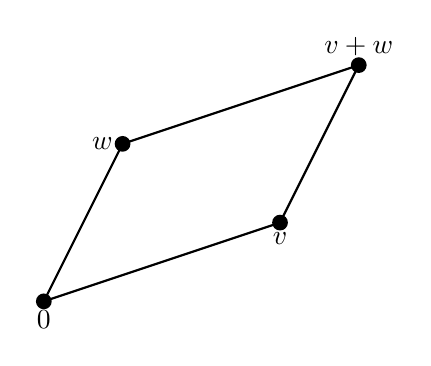
\begin{tikzpicture}[scale=1pt]
      \draw[thick] (0,0) -- (3,1) node[below] {};
      \draw[thick] (0,0) -- (1,2) node[left] {};
      \draw[thick] (1,2) -- (4,3) node[above] {};
      \draw[thick] (3,1) -- (4,3) node[right] {};
      \fill (3,1) circle (0.1) node[below] {$v$};
      \fill (1,2) circle (0.1) node[left] {$w$};
      \fill (0,0) circle (0.1) node[below] {$0$};
      \fill (4,3) circle (0.1) node[above] {$v+w$};
    \end{tikzpicture}
  \end{figure}
 
 
  By the above discussion, $f$ sends this parallelogram 
  to another parallelogram whose vertices are 
  $0$, $f(v)$, $f(w)$, and $f(v+w)$. By the geometric 
  interpretation of vector addition, this means that 
  $f(v+w) = f(v)+f(w)$. A similar argument works for 
  subtraction.

  Now, if $w\in \mathrm{Span}(v)\cap U$, then choose some 
  $u\in U\ssm \mathrm{Span}(v)$, and apply the above argument to 
  the pair $w-u$ and $v+u$, and then to the pairs 
  $w,u$ and $v,u$ to get $f(v+w) = f(v) + f(w)$.

  Let $v\in U\ssm \{0\}$ and $\alpha \in \R\ssm 0$ be such that 
  $\alpha v\in U$. We can write $f(\alpha v) = g(\alpha,v)f(v)$, and
  we need to show that $g$ does not depend on $v$. Let
  $w\in U\ssm \mathrm{Span}(v)$ be such that $\alpha w\in U$, 
  and consider the following line configuration:
  \begin{figure}[!h]
    \centering
    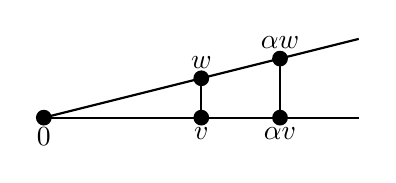
\begin{tikzpicture}
      \draw[thick] (0,0) -- (4,0) node[below] {};
      \draw[thick] (0,0) -- (4,1) node[left] {};
      \draw[thick] (2,0) -- (2,0.5) node[above] {};
      \draw[thick] (3,0) -- (3,0.75) node[above] {};
      \fill (0,0) circle (0.1) node[below] {$0$};
      \fill (2,0.5) circle (0.1) node[above] {$w$};
      \fill (2,0) circle (0.1) node[below] {$v$};
      \fill (3,0.75) circle (0.1) node[above] {$\alpha w$};
      \fill (3,0) circle (0.1) node[below] {$\alpha v$};
    \end{tikzpicture}
  \end{figure}


  Where the lines $(v,w)$ and $(\alpha v,\alpha w)$ are parallel. 
  Since $f$ preserves line configurations and paralellism, if 
  $f(\alpha v) = \beta f(v)$, then 
  $f(\alpha w) = \beta f(w)$. The case when 
  $w\in \mathrm{Span}(v)$ is treated similarly to additivity. 
  Overall, we get that $g$ as defined above 
  does not depend on $v$.

  Moreover, it is easy to check that wherever 
  $g$ is defined, $g(\alpha+\beta) = g(\alpha) + g(\beta)$ 
  and $g(\alpha\beta) = g(\alpha)g(\beta)$, and hence 
  is a restriction of a field 
  automorphism of $\R$, and hence is the identity.
\end{proof}
Note that we have actually proved a stronger result 
for a general field:
\begin{theorem}
  Let $\K$ be a field with at least three elements, and 
  let let $n>1$. Let $f:\K^n\to \K^n$ be a bijection sending 
  affine subspaces to affine subspaces. Then 
  there exists $z\in \K^n$ such that for all 
  $x,y\in \K^n$ and $\alpha\in \K$,
  \begin{align*}
    f(\alpha x + y) = g(\alpha)f(x) + f(y) + z
  \end{align*}
  Where $g:\K\to\K$ is a field automorphism.

  Such a function is called \textit{semilinear}
\end{theorem}
We can prove this by taking $U = \K^n$ and following the same argument. 
The condition $|\K|\ge 3$ is to be able to characterize 
parallel lines as disjoint lines lying in the same affine plane.

Using this, we can complete the construction of the main tool of this
section -- that any map projection which preserves convex sets can be
written as the composition of the gnomonic projection and an affine
linear transformation of the plane.

\begin{theorem}
  Let $\psi:U\to \R^2$ be a map projection 
  defined on a subset of the lower-hemisphere, and let 
  $\vphi$ be the gnomonic projection. If $\psi^{-1}$ sends 
  convex sets to convex sets, then there exists an affine linear map 
  $L$ such that $\psi = L\circ \vphi$.
\end{theorem}
\zs{this field automorphism business feels a little too abstract for the audience. In order to show $f$ is linear, you need to show $f(u+v) = f(u)+f(v)$ and $f(kx) = kf(x)$ and preserving parallelograms is strong enough to imply both of these. You showed additivity, and scaling is even easier. If a parallelogram is preserved, it sends parallel segments of equal length to parallel segments of equal length, and this extends to the statement that any pair of parallel segments has the ratio of their lengths preserved, so any pair of collinear segments have the ratio of their length preserved, which implies linear.}
\begin{proof}
  By Lemma ~\ref{lem:gnomonic_convex}, the map $\vphi\circ
  \psi^{-1}:\psi(U)\to \R^2$ sends convex sets to convex sets. It is
  bijective on its range, since $\psi$ and $\vphi$ are bijective, and
  hence satisfies the conditions of Theorem
  ~\ref{thm:geometric_algebra}, meaning that there exists an affine
  linear isomorphism $L^{-1}:\R^2\to \R^2$ such that $\vphi = \psi
  \circ L^{-1}$.  Thus, $\psi = \vphi \circ L$, as desired.
  \mute{
  By the previous lemma, the gnomonic projection does indeed preserve
  convex sets.   If a map projection preserves convex sets, it must in
  particular preserve the one-dimensional convex sets, meaning it maps
  segments of great circles on the sphere to line segments in the
  plane.  Take $\psi$ and $\varphi$ to convexity-preserving map
  projections, and, without loss of generality take $\varphi$ to be
  the standard gnomonic projection described above. We consider the
  composition $\psi\varphi^{-1}$, which is a transformation of the
  plane which preserves convex sets, so in particular it sends line
  segments to line segments.  Since these transformations also
  preserve containment, we can additionally observe that
  $\psi\varphi^{-1}$ preserves \textit{collinearity} in the plane,
  which means it is an affine linear transformation of the plane.
  Since we can write $\psi$ as $\psi\varphi^{-1}\varphi$, we have
  successfully written our convexity-preserving map as the composition
  of the gnomonic projection and an affine linear transformation of
  the plane.}
\end{proof}
\zs{we don't use this anywhere. it's cute, but I don't think it's relevant}



\subsection{Stereographic Projection}

\zs{defn 9, lem 5 lem 6 lem 7 lem 8}

\begin{definition}
  The \textbf{stereograpic projection} from the sphere to the plane is
  defined by placing the plane tangent to the sphere at the south
  pole, and for any point $p$ on the sphere other than the north pole,
  $p$ is sent to the unique point $q$ in the plane which is on the
  line in 3-space passing through the north pole and $p$.

  If $(x,y,z)$ is a point on the sphere, then the action of the
  stereographic projection is
  \begin{align*}
    (x,y,z)\mapsto \left(\frac{x}{1-z},\frac{y}{1-z}\right)
  \end{align*}
  and its inverse, for $(u,v)$ in the plane:
  \begin{align*}
    (u,v)\mapsto \left( \frac{2u}{1+u^2+v^2},\frac{2v}{1+u^2+v^2},
    \frac{u^2+v^2-1}{1+u^2+v^2}   \right)
  \end{align*}
\end{definition}

What is somewhat surprising is that this projection sends every cap on
the sphere which doesn't pass through the north pole to a circle in
the plane.  There are several proofs of this fact, and we present
a rather straightforward algebraic one here.

\abn{This is a fact that is usually taught at a second 
year complex analysis course - perhaps we can leave this out if 
we want to conserve space?}
\begin{lemma}
  The stereographic projection sends every cap which does not pass through the north pole to a circle in the plane.
\end{lemma}
\begin{proof}
  We proceed algebraically.  Since a cap on the sphere can be
  identified by the plane in $\R^3$ which intersects the sphere along
  its boundary, we can parametrize such a cap by writing the equation
  for its corresponding plane, $ax+by+cz=d$, restricting $(x,y,z)$ to
  be points on the sphere.  The image in the plane of this cap is some
  set of $(u,v)$ points, and we can explicitly write this by
  substituting in for $x$, $y$, and $z$ the corresponding values for
  the inverse stereographic projection.  We write
  $\mathcal{W}=u^2+v^2$ for the ease of presentation. 

  \begin{align*}
    d&=ax+by+cz\\
    d&=a\left(\frac{2u}{1+u^2+v^2}\right)+b\left(\frac{2v}{1+u^2+v^2}\right)+c\left(\frac{u^2+v^2-1}{1+u^2+v^2}\right),
    \text{ by substitution}\\
    d&=a\left(\frac{2u}{1+\mathcal{W}}\right)+b\left(\frac{2v}{1+\mathcal{W}}\right)+c\left(\frac{\mathcal{W}-1}{1+\mathcal{W}}\right),
    \text{ by change-of-variable }\mathcal{W}=u^2+v^2\\
    d\left(1+\mathcal{W}\right)&=2au+2bv+c\left(\mathcal{W}-1\right),
    \text{ multiplying through by }1+\mathcal{W}\\ 0 &=
    (c-d)\mathcal{W} + 2au +2bv - c - d,\text{ by rearrangement}\\
    0 &= (c-d)(u^2+v^2)+2au+2bv - c - d,\text{ by change-of-variable
    } \mathcal{W}=u^2+v^2 
  \end{align*}

  This last step is the equation of a circle in the plane if $c\neq d$
  and a line otherwise.  Since $c=d$ if and only if the point
  $(x,y,z)=(0,0,1)$ (i.e. the north pole) is on the plane, and we
  assumed that this is not the case, we have shown that the image
  under the stereographic projection of every cap which does not pass
  through the north pole is a circle in the plane.

\end{proof}

We have in-hand a circle-preserving map projection, and we now
turn to demonstrating that the stereographic projection is essentially
the unique map projection with this property.  We can observe that if
we perform stereographic projection and compose it with
a transformation of the plane which sends every circle to a circle,
then this composition is a circle-preserving map projection.  The next
lemma demonstrates that the class of transformations of the plane
which preserve circles is actually quite narrow.
\abn{Localized the lemma to concern mobius transformations}
\mute{
\begin{lemma}
  If $T$ is a transformation of the plane which sends every circle in
the plane to another circle, then $T$ must be a linear transformation
which is the composition of a scaling, a rotation, a reflection, and
a translation, i.e. a scaled isometry.  
\end{lemma}
\begin{proof}

  We first argue that if we restrict our attention to \textit{linear}
  transformations, the scaled isometries are the only transformations
  which preserve circles.  

  If $T$ is a scaled isometry with scaling factor $\alpha$, then, by
  definition, for any points $x$ and $y$, the distance between $T(x)$
  and $T(y)$ is $\alpha$ times the distance between $x$ and $y$.
  Therefore, if we choose a circle $Y$ of radius $r$ and let $x$ be
  the center, then for any $y\in Y$, $d(T(x),T(y)) = \alpha r$, so
  $T(Y)$ is a circle of radius $r$.

  Next, if $T$ is a linear transformation which is \textit{not}
  a scaled isometry, then we can find three points $x$, $y$, and $z$
  such that $d(T(x),T(y)) = \alpha d(x,y)$ but $d(T(x),T(z)) \neq
  \alpha d(x,z)$.  Furthermore, since linear transformations preserve
  ratios of lengths of collinear segments, and we have two segments
  whose ratios of lengths are not preserved, these three points cannot
  be collinear, so we can consider the circle centered at $x$ and
  passing through $y$ and $z$.  But, since the ratio of lengths isn't
  preserved, $T$ distorts this circle, so $T$ is not
  circle-preserving.

  We next need to rule out the existence of a non-linear
  transformation $T$ which is circle preserving.  We proceed by
  contradiction.  Suppose that $T$ is non-linear and
  circle-preserving.  Then, since $T$ is non-linear, there is some
  line $\ell$ such that the image $T(\ell)$ is not a line, so we can
  find three points $x$, $y$, and $z$ which are collinear, but $T(x)$,
  $T(y)$, and $T(z)$ are not.  Therefore, we can find a unique circle
  $C_T$ passing through $T(x)$, $T(y)$, and $T(z)$.  Let $T(a)$ be
  some other point on this circle, and we consider the preimage of
  this point, $a$.  If $a$ is not on the line $\ell$, then we can
  construct two circles, one passing through $a$, $x$, and $y$ and one
  passing through $a$, $y$, and $z$.  These two circles intersect at
  only two points, $a$ and $y$, but both of these circles are sent to
  $C_T$ by $T$, which is impossible if $T$ is injective.  Therefore,
  $a$ must lie on the line $\ell$.

  By repeating this argument, any point on the circle $C_T$ must be
  the image of some point on $\ell$.  By continuity, we can see that
  every point on $\ell$ is sent to a point on $C_T$, but the
  homeomorphic image of a line cannot be a circle, so such
  a non-linear $T$ cannot exist.

  Thus, a transformation of the plane is circle-preserving if and only
  if it is a scaled isometry.
\end{proof}
\zs{here is where the local mobius thing should go.  if it's a two-sentence technicality (i.e. our proof is ``Suppose we were only interested in circle-preserving maps in \textit{regions} of the plane. Then, we should want every \textit{circular arc} in the patch to be sent to a circular arc in the image and everything carries through as before, since three non-collinear points define a circular arc when restricted to a patch'', then it can even just be a footnote.})
We can put these two pieces together to prove the main tool of this
section -- that any map projection from the sphere to the plane which
preserves circles is the composition of the stereographic projection
and a scaled isometry.
}
\begin{lemma}
  Let $f:U\to V$ be a bijection between two planar regions 
  sending generalised circles to generalised circles. 
  Then $f$ is a M\"{o}bius transformation composed with a 
  reflection.
\end{lemma}
This gives us a surprisingly useful theorem:
\begin{theorem}\label{thm:stereographic_mobius}
  The map projections from the sphere to the plane which send every
  cap to a circle are exactly those which can be written as the
  composition of the stereographic projection followed by a 
  M\"{o}bius transoformation and a reflection.
\end{theorem}
\begin{proof}
  Let $\varphi$ and $\psi$ be two map projections which preserve
  circles, and without loss of generality let $\varphi$ be the
  standard stereographic projection.  Then the composition
  $M^{-1}=\psi\circ\varphi^{-1}$ is a transformation of 
  the plane which preserves circles, so by the previous lemma, 
  $M^{-1}$ is a M\"{o}bius transformation composed with a reflection. 
  Then, we can write $\psi= M\varphi$, which is the
  composition of the stereographic projection and a scaled isometry.
\end{proof}

\zs{not convinced we need this next bit anymore}
\abn{I muted it}
\mute{
As in the previous section, we can construct an example of two regions
whose Reock scores are permuted by the stereographic projection.  In
fact, we can use \textit{exactly} the same pair of regions as in the
convex hull settings, as is made clear by the following lemma.

\begin{lemma}
  Let $\varphi$ be the stereographic projection and $C_\theta$ be
  a spherical cap centered at the south pole parametrized by the angle
  $\theta <\pi/4$ formed between the central axis of the sphere and
  the line of projection passing through the north pole and the
  boundary of the cap (Figure~\ref{fig:stereocap}). Then
  $\vphi(C_\theta)$ is a disk in the plane, centered at the origin, and
  has radius $2\tan\theta$
\end{lemma}
\begin{figure}
  \centering
  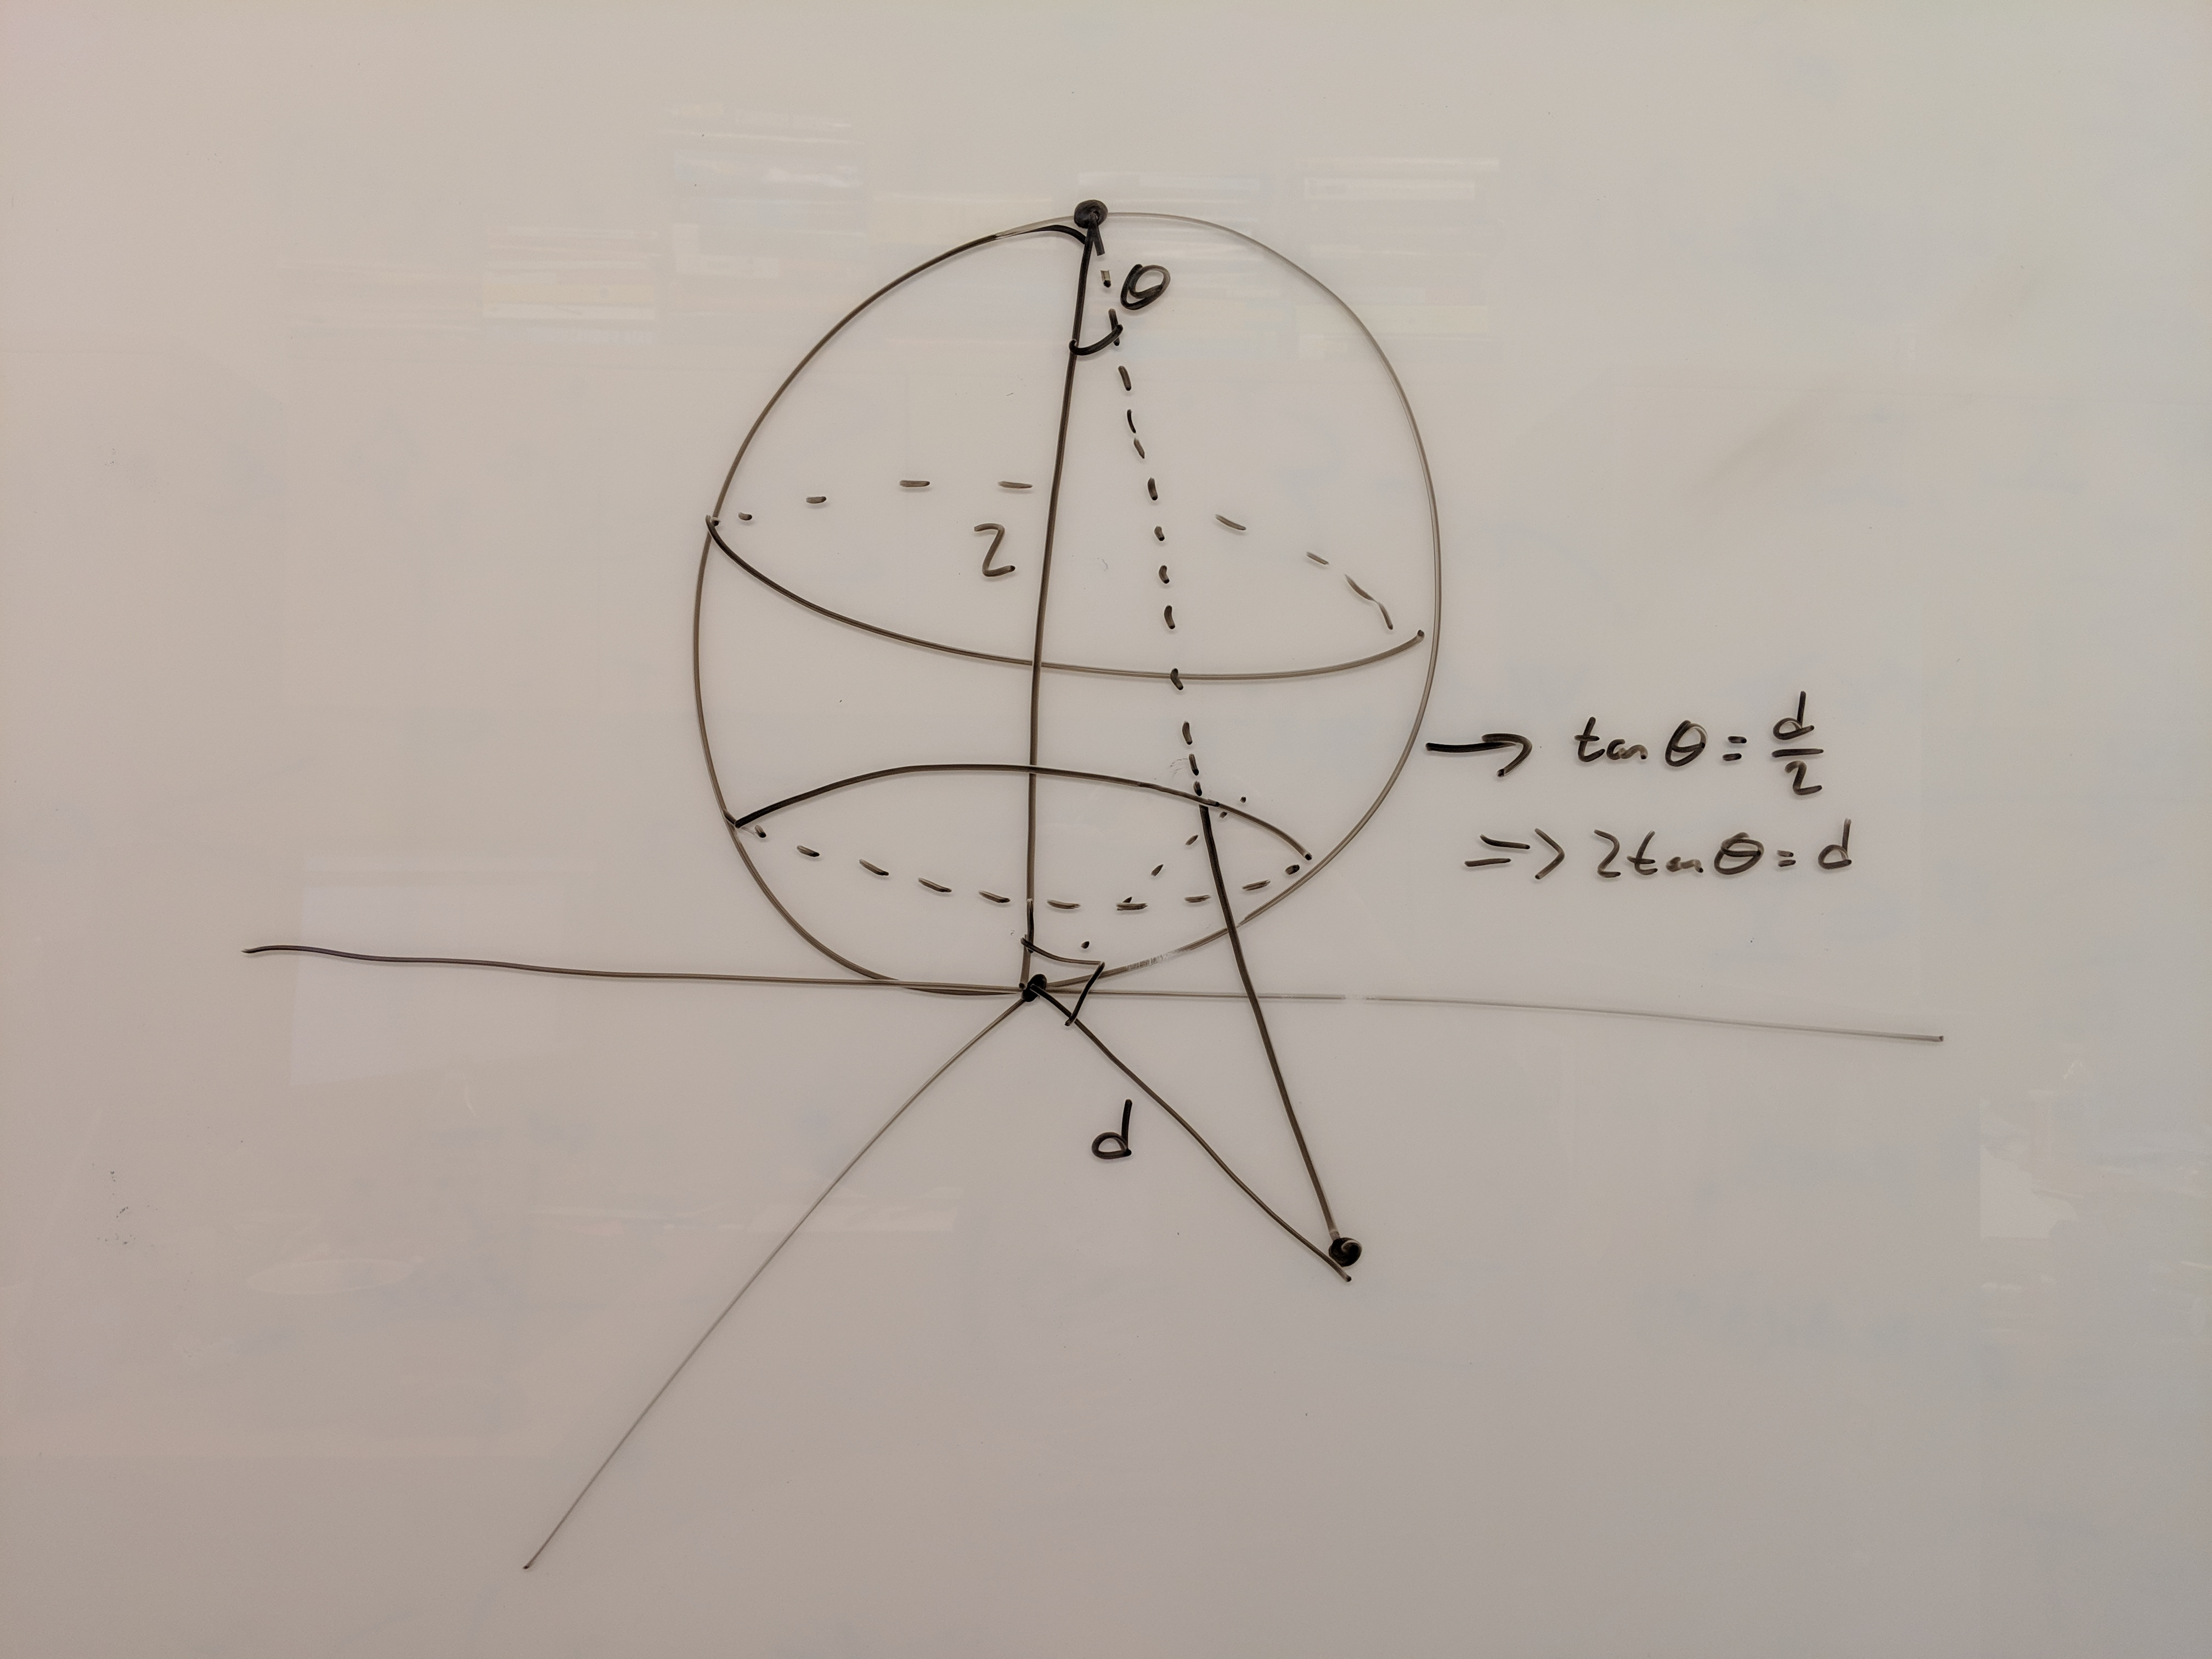
\includegraphics[width=.8\textwidth]{figs/stereo_cap.jpg}\\
  \caption{ The image of a cap with angle $\theta$ between the polar axis and the line of projection is a circle of radius $2\tan\theta$.  }
  \label{fig:stereocap}
\end{figure}
\begin{proof}


  Since $\varphi$ projects from the north pole of the sphere and the
  sphere's south pole is mapped to the origin in the plane, the image
  of $C_\theta$ is totally radially symmetric about the origin, and is
  therefore a circle.  To see that its radius is $2\tan(\theta)$,
  place the south pole of the sphere tangent to the plane at the
  origin. By construction, for any point $p$ on the boundary of
  $C_\theta$, there is a unique line passing through the north pole of
  the sphere, $p$, and the point $\varphi(p)$ on the boundary of the
  disk in the plane.  By definition, this line meets the central axis
  of the sphere at an angle of $\theta$, and the central axis of the
  sphere meets the plane orthogonally, so the center of the sphere,
  the origin, and the point $\varphi(p)$ form a right triangle with
  angle $\theta$.  Since we know that the distance between the north
  pole of the sphere and the origin is 2, we can write the distance
  between the origin and $\varphi(p)$ as $2\tan(\theta)$.

\end{proof}
\zs{$\backslash${end} not convinced}
}
